\chapter{Introduction}

\section{Course Structure}
\twosplit{
	\begin{center}
		\begin{tikzpicture}
			\clip (0,0)  circle (2cm) ;
			\node[anchor=center] at (0,-0.5) {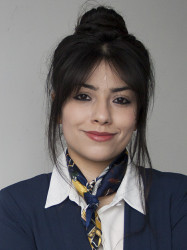
\includegraphics[width=4.5cm]{introduction/images/azalea_raad.jpg}};
		\end{tikzpicture}
		\centerline{\textbf{Dr Azelea Raad}}
	\end{center}
	\textbf{First Half}
	\begin{itemize}
		\item The while language
		\item Big \& small step semantics
		\item Structural induction
	\end{itemize}
}{
	\begin{center}
		\begin{tikzpicture}
			\clip (0,0)  circle (2cm) ;
			\node[anchor=center] at (-.1,0.0) {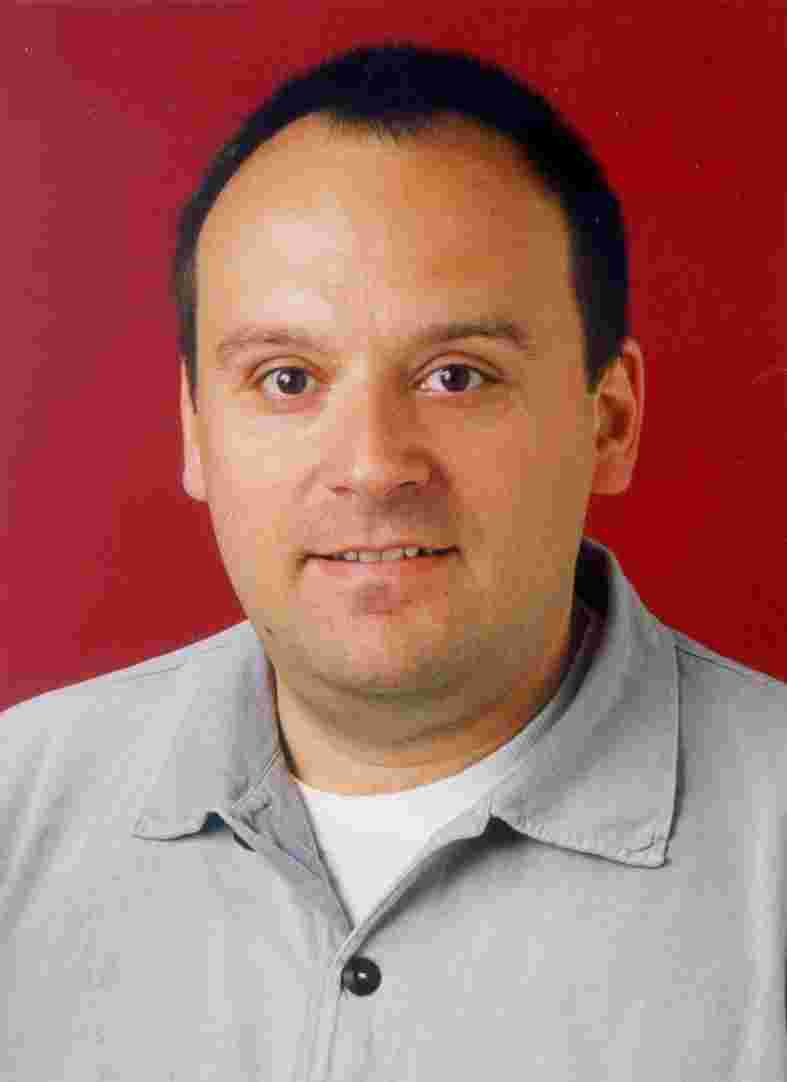
\includegraphics[width=4.5cm]{introduction/images/herbert_wiklicky.jpg}};
		\end{tikzpicture}
		\centerline{\textbf{Dr Herbert Wiklicky}}
	\end{center}
	\textbf{Second Half}
	\begin{itemize}
		\item Register Machines \& gadgets
		\item Turing Machines
		\item Lambda Calculus
	\end{itemize}
}

\section{Algorithms}
\begin{sidenotebox}{Euclid's Algorithm}
    Algorithm to find the greatest common divisor published by greek mathematician Euclid in $\approx 300$ B.C.
    \inputminted{haskell}{introduction/code/euclid.hs} 
\end{sidenotebox}
\begin{sidenotebox}{Sieve of Eratosthenes}
    Used to find the prime numbers within a limit. Done by starting from the 2, adding the number to the primes, marking all multiples as non-prime, then repeating progressing to the next non-marked number (a prime) and repeating. 
    \\
    \\ The sieve is attributed to Eratosthenes of Cyrene and was first published $\approx 200$ B.C.
    \inputminted{haskell}{introduction/code/eratosthenes.hs}
\end{sidenotebox}
\begin{sidenotebox}{Al-Khwarizmi}
    A persian polymath who first presented  systematic solutions to linear and quadratic equations (by completing the square). 
    He pioneered the treatment of algebra as an independent discipline within mathematics and introduced foundational methods such as the notion of balancing \& reducing equal equations (e.g subtract/cancel the same algebraic term from both sides of an equation)
    \\
    \\ His book title \RL{الجبر} \textit{"al-jabr"}  resulted in the word \textit{algebra} and subsequently algorithm.   
\end{sidenotebox}

Algorithms predate the computer, and have been studied in a mathematical/logical context for centuries.
\begin{itemize}
    \item Very early attempts such as the Antikythera Mechanism (an analogue calculator for determining the positions of ) 
    \item Simple configurable machines (e.g automatic looms, pianola, census tabulating machines) invented in the 1800s.
    \item Basic calculation devices such as Charles \textit{Babbage's Difference Engine} further generalised the idea of a calculating machine with a sequence of operations, and rudimentary memory store.
    \item Babbage's Analytical Engine is generally considered the world's first digital computer design, but was not fully implemented due to the limits of precision engineering at the time.
    \item English mathematician Ada Lovelace writes the first ever computer program  (to calculate bernoulli numbers) on Babbage's analytical engine.
\end{itemize}

\begin{sidenotebox}{Note G}
    While translating a french transcript of a lecture given by Charles Babbage at the University of Turin on his analytical engine, Ada Lovelace added several notes (A-G), with the last including a description of an algorithm to compute the \href{https://en.wikipedia.org/wiki/Bernoulli_number}{Bernoulli numbers}.
    \begin{center}
        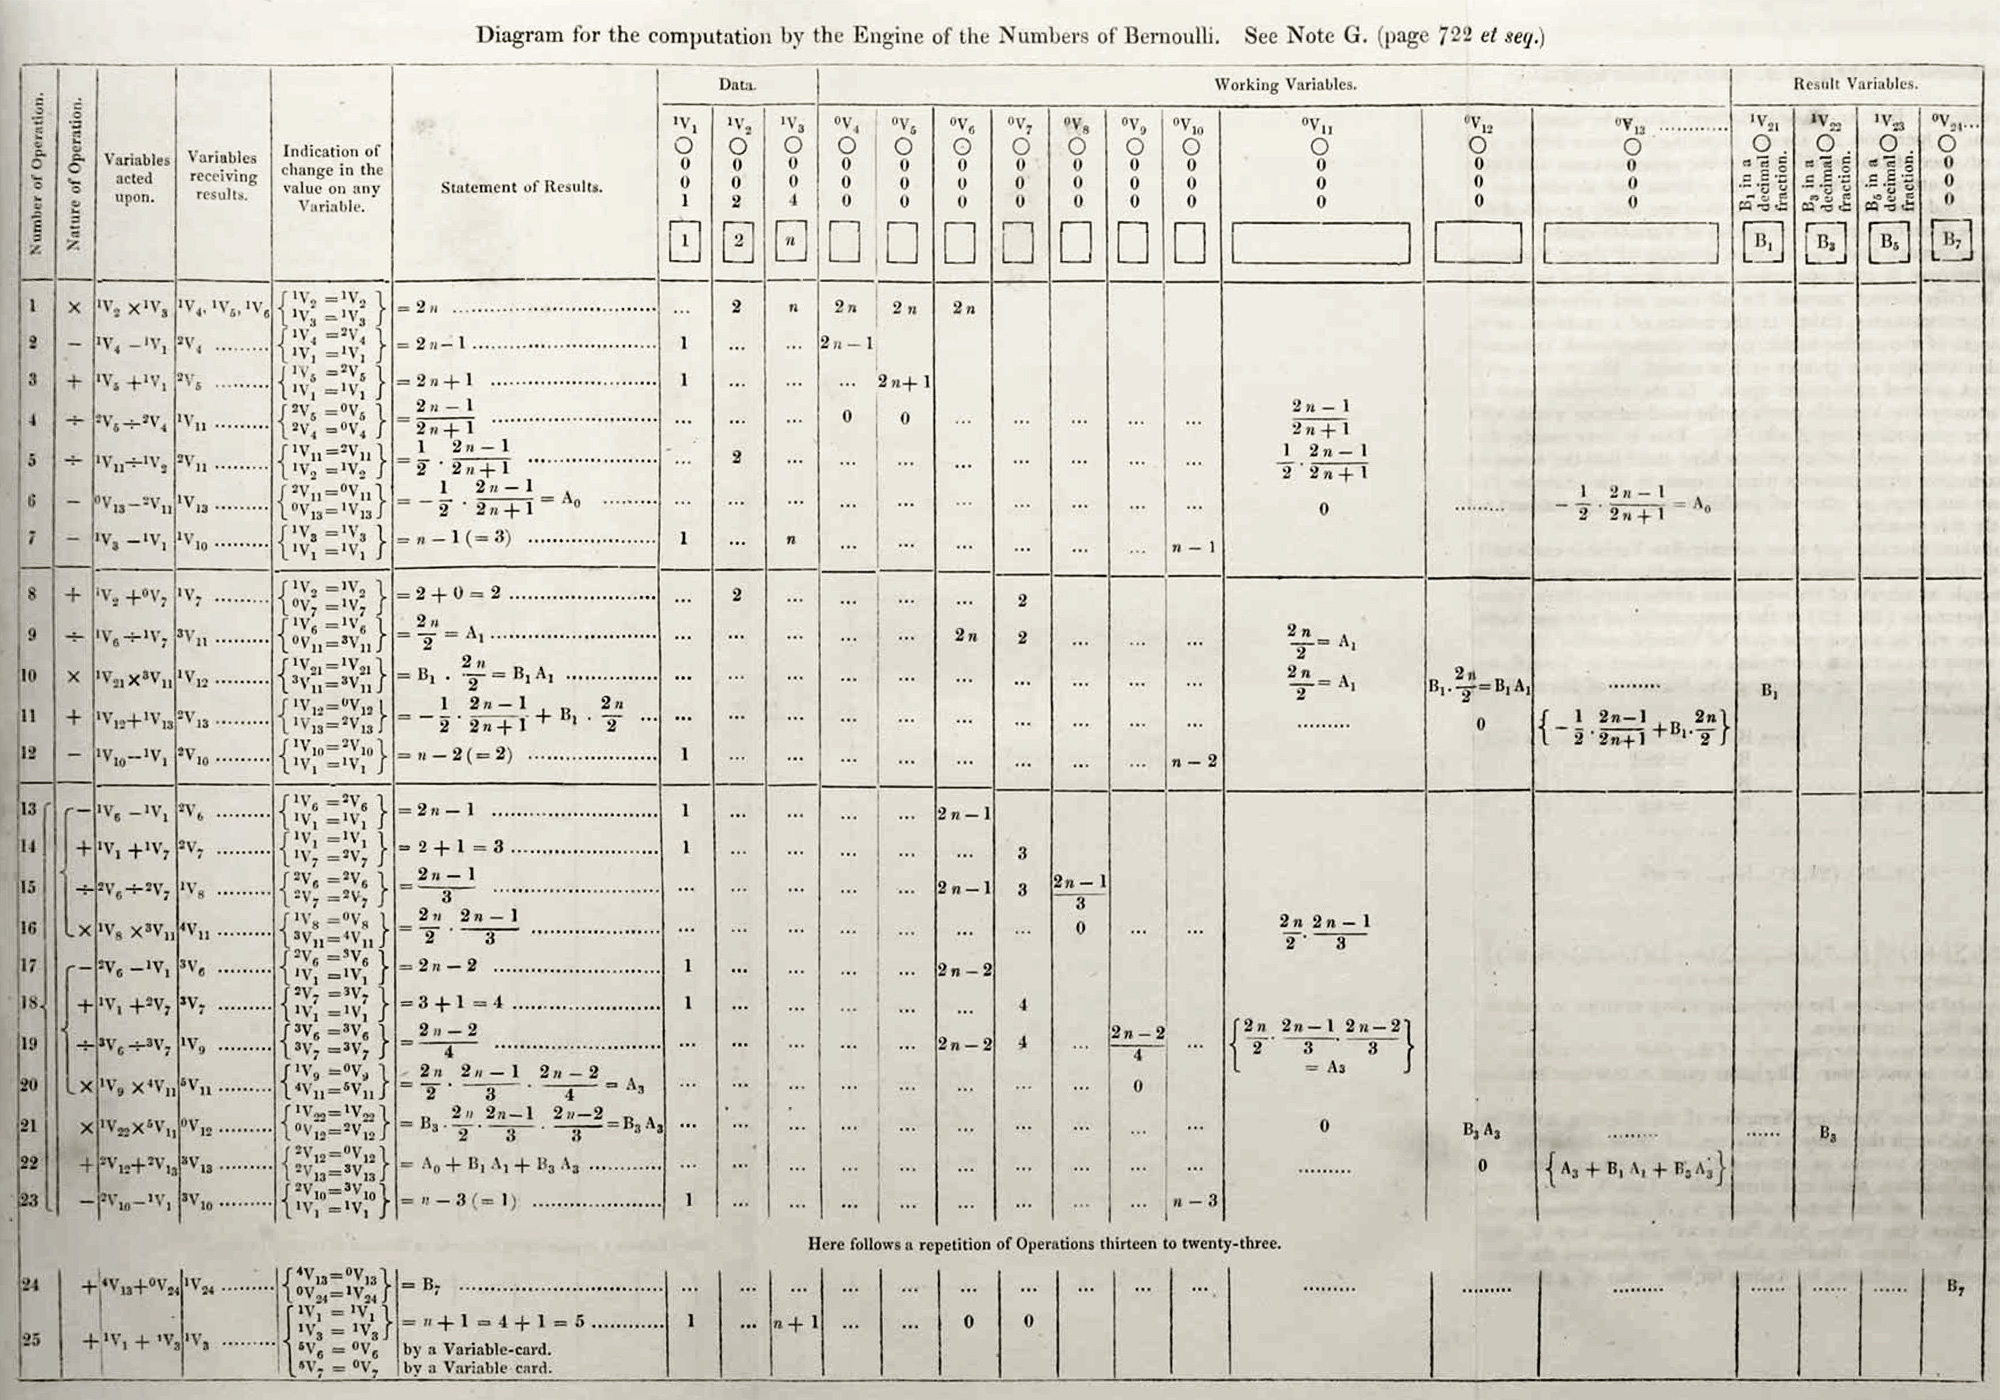
\includegraphics[width=.8\textwidth]{introduction/images/note_G.jpg}
    \end{center}
\end{sidenotebox}

\begin{sidenotebox}{Babbage's Machines}
    The \textit{Difference Engine} was used as the basis for designing the fully programmable \textit{Analytical Engine}.
    \begin{itemize}
        \item Held back by lack of funds, limitations of precision machining at the time.
        \item Contains an ALU for arithmetic operations, supports conditional branches and has a memory
        \item Part of the machine (including a printing mechanism) are on display at the science museum.
    \end{itemize}
\end{sidenotebox}

\section{Decision Problems}
\begin{definitionbox}{Formulas}
    Well formed logical statements that are a sequence of symbols form a given formal language. e.g $(p \lor q) \land i$ is a formula, but $) \lor \land j i$ is not.
\end{definitionbox}
Given:
\begin{itemize}
	\item A set $S$ of finite data structures of some kind (e.g formulae in first order logic).
	\item A property $P$ of elements of $S$ (e.g the porperty of a formula that it has a proof).
\end{itemize}
The associated decision procedure is:
\\
\\ Find an algorithm such that for any $s \in S$, if $s$ has property $P$ the algorithm terminates with $1$, otherwise with $0$.

\subsection{Hilbert's Entscheidungsproblem}
\begin{quote}
    \textit{Is there an algorithm which can take any statement in first-order logic, and determine in a finite number of steps if the statement is provable?}
\end{quote}
\begin{definitionbox}{First Order Logic/Predicate Logic}
    An extension of propositional logic that includes quanifiers ($\forall, \exists$), equality, function symbols (e.g $\times, \div, +, -$) and structured formulas (predicate functions).
\end{definitionbox}

\noindent This problem was originally presented in a more ambiguous form, using a logic system more powerful than first-order logic.
\\
\\ '\textit{Entscheidungsproblem}' means 'decision problem'
\\
\\ Many tried to solve the problem, without success. One strategy was to try and disprove that such an algorithm can exist.
In order to answer this question properly a formal definition of algorithm was required.
\section{Algorithms}
\subsection{Algorithms Informally}
Common features of Algorithms:
\begin{center}
    \begin{tabular}{l p{.8\textwidth}}
        \textbf{Finite} & Description of the procedure in terms of elementary operations. \\
        \textbf{Deterministic} & If there is a next step, it is uniquely determined - that is on the same data, the same steps will be made. \\
        \textbf{Terminate?} & Procedure may not terminate on some input data, however we can recognize when it terminates and what the result is. \\
    \end{tabular}
\end{center}
\noindent
In 1935/35, Alan Turing (Cambridge) and Church (Princeton) independently gave negative soltuions to Hilberts Entscheidungsproblem (showed such an algorithm could not exist).
\begin{enumerate}
	\item They gave concrete/precise definitions of what algorithms are (Turing Machines \& Lambda Calculus).
	\item They regarded algorithms as data, on which other algorithms could act.
	\item They reduced the problem to the \textit{Halting problem}.
\end{enumerate}
This work led to the Church-Turing Thesis, that shows everything computable is computed by a Turing Machine. Church's Thesis extended this to show that General Recurisve Functions were the same type as those expressed by lambda calculus, and Turning showed that lambda calculus and the turning machine were equivalent.

\subsubsection{Algorithms Formalised}
Any formal definition of an algorithm should be:
\begin{center}
    \begin{tabular}{l p{.8\textwidth}}
        \textbf{Precise} & No ambiguities, no implicit assumptions, Should be phrased mathematically. \\
        \textbf{Simple} & No unnecessary details, only the few axioms required. Makes it easier to reason about. \\
        \textbf{General} & So all algorithms and types of algorithms are covered. \\
    \end{tabular}
\end{center}

\subsection{The Halting Problem}
The \textit{Halting problem} is a \textit{decision problem} with:
\begin{itemize}
	\item The set of all pairs $(A,D)$ such that $A$ is an algorithm, and $D$ is some input datum on which the algorithm operates.
	\item The property $A(D)\downarrow$ holds for $(A,D) \in S$ if algorithm $A$ when applied to $D$ eventually produces a result (halts).
\end{itemize}
Turning and Church showed that there is no algorithm such that:
\[\forall (A,D) \in S \begin{bmatrix}
		H (A,D) & = & 1 & A(D)\downarrow \\
		        &   & 0 & otherwise
	\end{bmatrix}\]
The final step for Turing/Church's proof was to construct an algorithm encoding instances $(A,D)$ of the halting problem as statements such that:
\[\Phi_{A,D} \ is \ provable \leftrightarrow A(D)\downarrow\]

\subsection{Algorithms as Functions}
It is possible to give a mathematical description of a computable function as a special function between special sets.
\\
\\ In the 1960s Strachey \& Scott (Oxford) introduced \textit{denotational semantics}, which describes the meaning (denotation)
of an algorithm as a function that maps input to output.
\begin{definitionbox}{Domains}
	Domains are special kinds of partially ordered sets. Partial orders meaning there is an order of elements in the set, but not every element is comparable.
	\\
	\\ Partial orders are reflexive, transitive and anti-symmetric. You can easily represent them on a Hasse Diagram.
	\begin{center}
		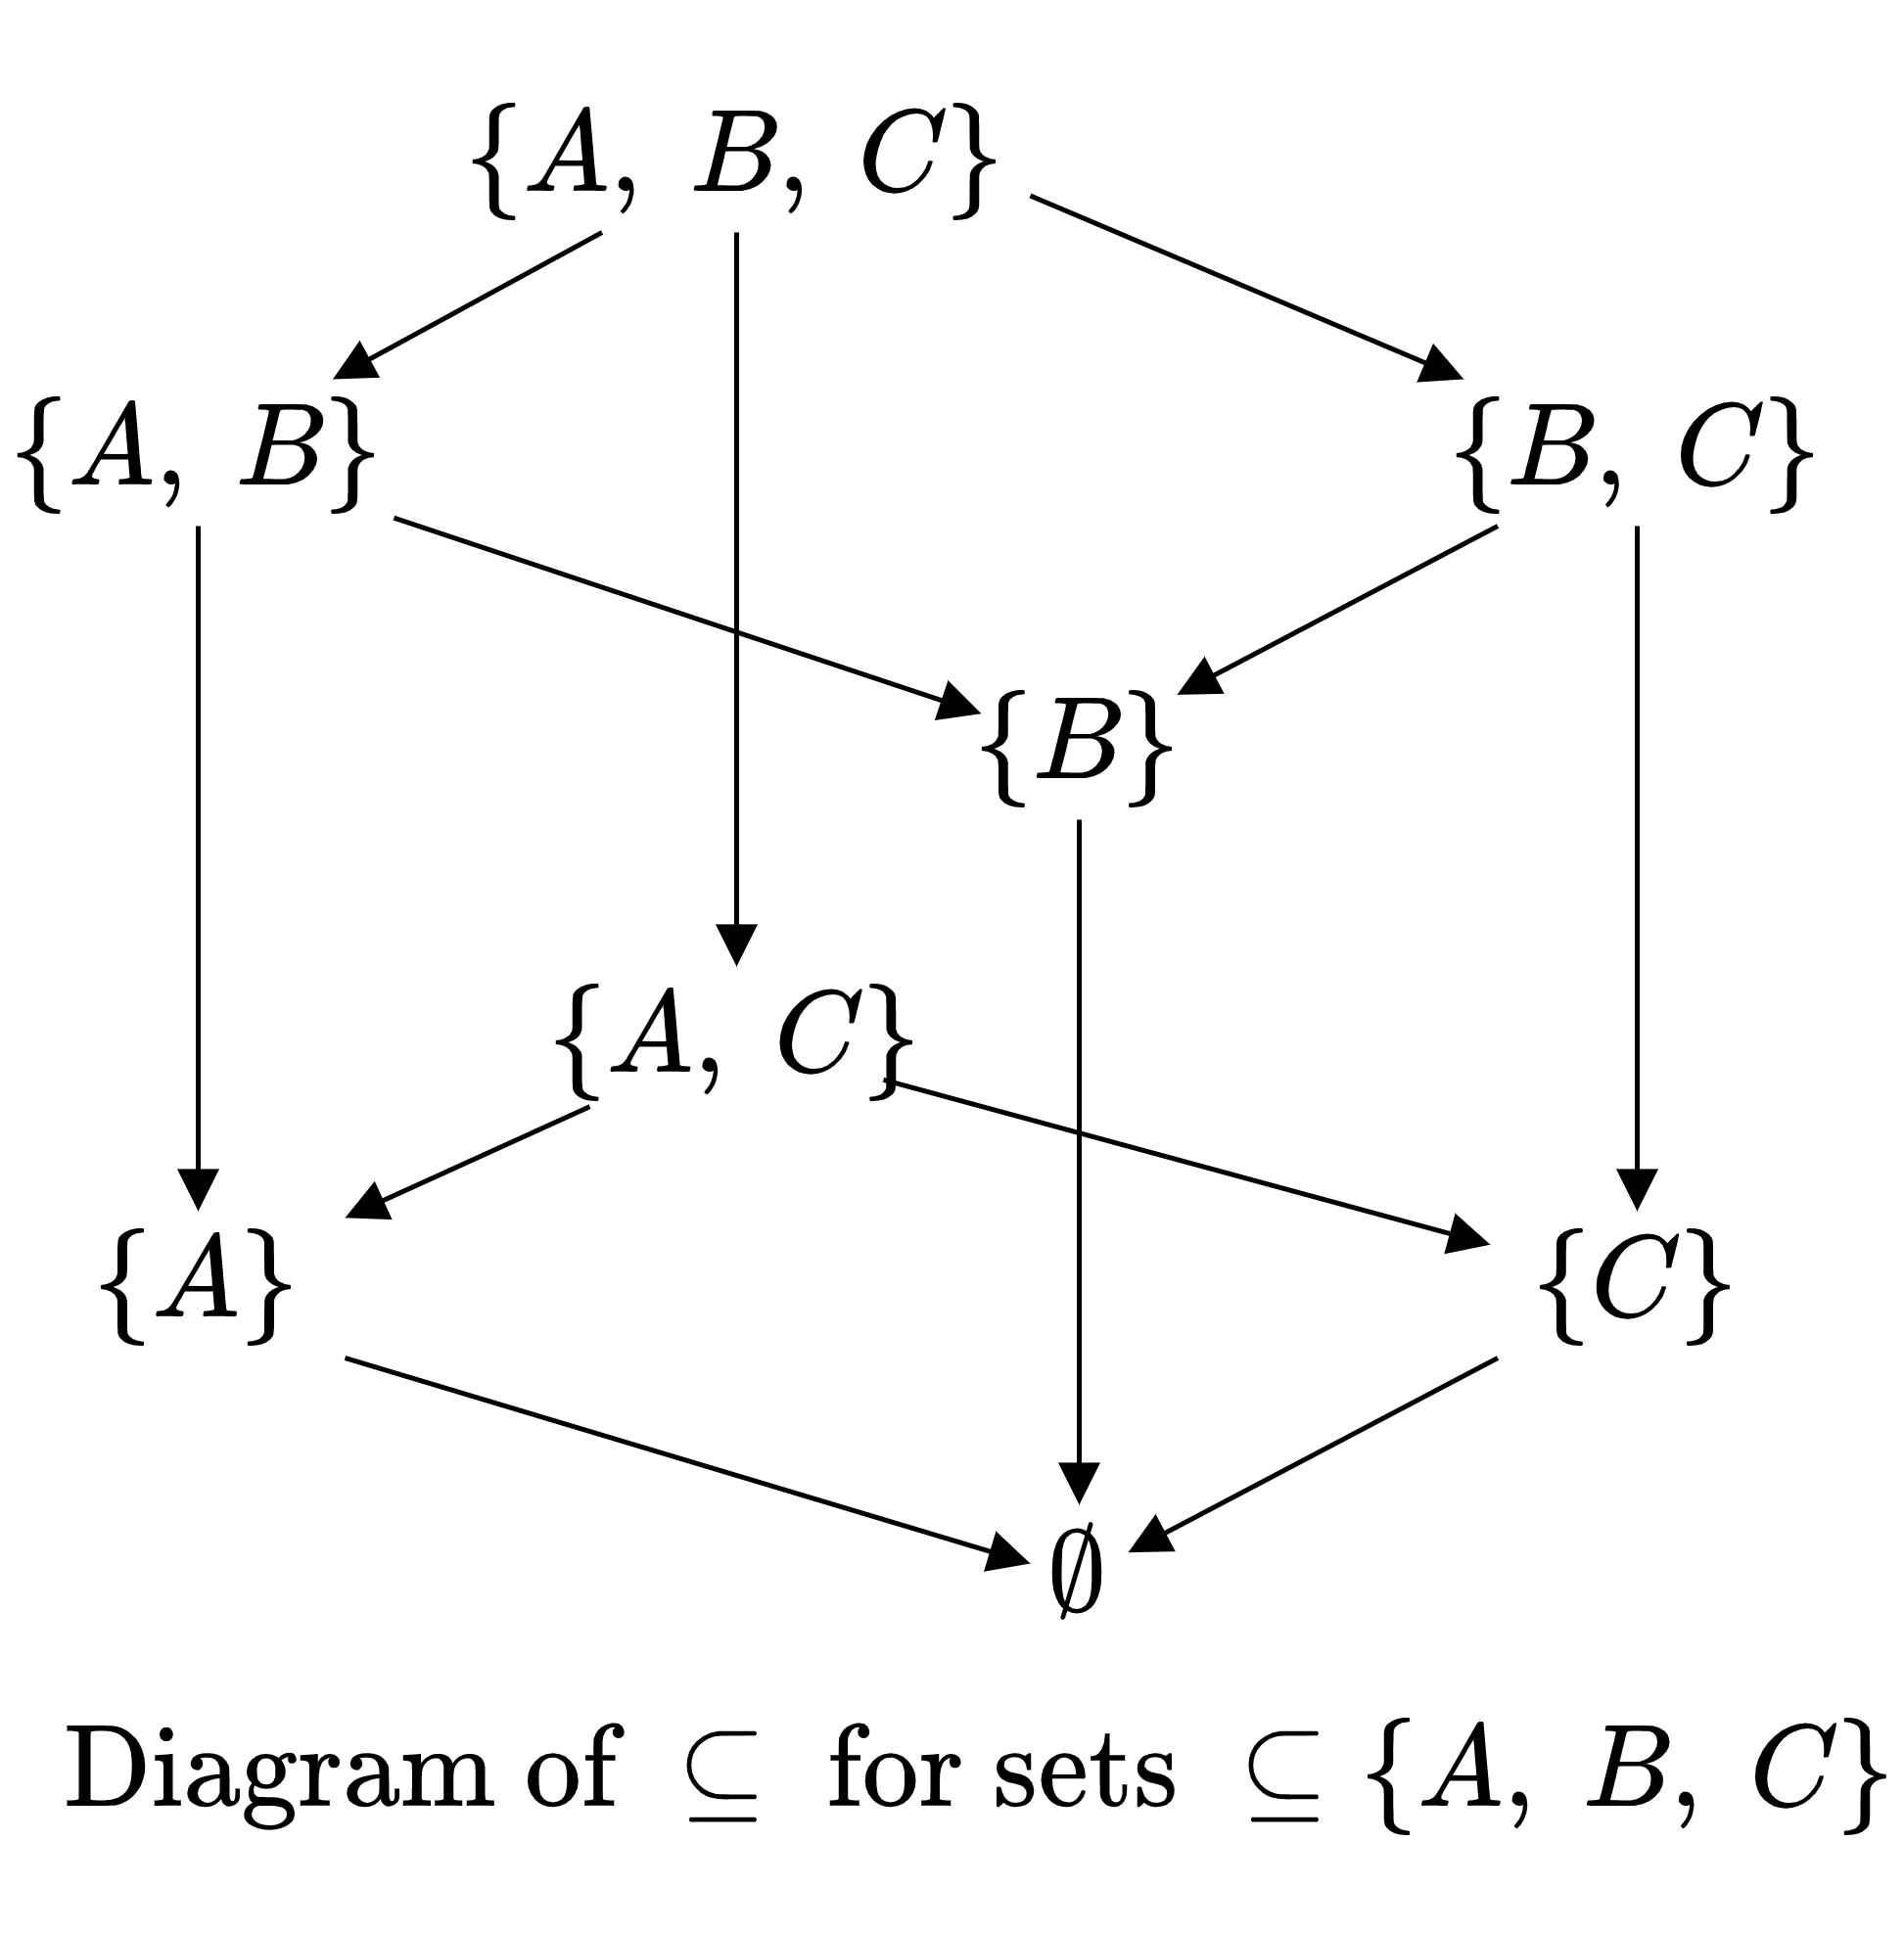
\includegraphics[width=.3\textwidth]{introduction/images/hasse_diagram.drawio.png}
	\end{center}
\end{definitionbox}
\noindent 
Scott solved the most difficult part, considering recursively defined algorithms as continuous functions between domains.

\subsection{Haskell Programs}
Example using a basic implementation of power.
\inputminted{haskell}{introduction/code/power.hs}

\newcommand{\step}[1]{$\leadsto$ \ #1\\}

\begin{minipage}{.5\textwidth}
	\textbf{O(n)} \\
	power 7 5 \\
	\step{7 * (power 7 4)}
	\step{7 * ( 7 * (power 7 3))}
	\step{7 * ( 7 * (7 * (power 7 2)))}
	\step{7 * ( 7 * (7 * (7 * (power 7 1))))}
	\step{7 * ( 7 * (7 * (7 * (7 * (power 7 0)))))}
	\step{7 * ( 7 * (7 * (7 * (7 * 1))))}
	\step{16807}
\end{minipage} \begin{minipage}{.5\textwidth}
	\textbf{O(log(n)) steps} \\
	power' 7 5 \\
	\step{7 * (power' 7 2)\^2}
	\step{7 * ((power' 7 1)\^2)\^2}
	\step{7 * ((7 * (power' 7 0)\^2)\^2)\^2}
	\step{7 * ((7 * (1)\^2)\^2)\^2}
	\step{16807}
\end{minipage}

These two functions are equivalent in result however operate differently (one much faster than the other).

\section{Program Semantics}
\begin{definitionbox}{Denotational Semantics}
    \begin{itemize}
        \item A program's meaning is described computationally using denotations (mathematical objects)
        \item A denotation of a program phrase is built from its sub-phrases.
    \end{itemize}    
\end{definitionbox}
\begin{definitionbox}{Operational Semantics}
    Program's meaning is given in terms of the steps taken to make it run.
\end{definitionbox}

\noindent There are also \textit{axiomatic semantics} and \textit{declarative semantics} but we will not cover them here.
